\scanpage{121}
a sort of geometrico-arithmetic synthesis of the numerous cohomological theories which one has\deleted{\unsure{rait}} at present for algebrai\deleted{\unsure{qu}}c varieties,\deleted{of all dimensions,}and of the linear representations of arithmetic \rlap{\deleted{g}}Galois groups to which these theories give rise\deleted{\unsure{s}}.

5) \uline{Solution of the problem of introducing a} $\handwritten{\lambda}$-\uline{structure} (corresponding to the notion of exterior power) \uline{in the ring} $K^\bullet(X)$\handwritten{(}called ``Grothendieck's''\handwritten{)}of a locally ringed topological space (for example an analytic variety, or\deleted{\unsure{nd|md}} a differe\rlap{\deleted{\unsure{t}}}nti\rlap{\deleted{b}}a\rlap{\deleted{\unsure{a}}}ble manifold, or a scheme)\handwritten{,} constructed with the aid of the category of ``perfect'' complexes on $X$. This problem was pointed out as the most important problem \mbox{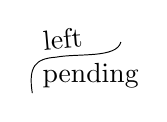
\begin{tikzpicture}[x=1em,y=1em,baseline=(b.base)]
\node[anchor=base west,inner sep=0] (b) at (0,0) {pending};
\node[anchor=base west,inner sep=0,rotate=5] at (.05,1.15) {\inserted{\handwritten{left}}};
\draw[line width=.35pt] (-.35,-.4) .. controls (-.5,.55) and (-.25,.85) .. (.5,.9) .. controls (1.3,1.05) and (2.7,.85) .. (2.85,1.45);
\end{tikzpicture}} in the 1966/67 Algebraic Geome\rlap{\deleted{y}}\handwritten{t}ry Seminar at the Institute for Advanced Scientific Studies, on the Riemann-Roch theorem. The necessity of working with the $K^\bullet(X)$ defined in terms of perfect \uline{complexes}, rather than only vector \uline{bundles}, is \unsure{imposed|imposed} by \deleted{nécess} incontestable technical imperatives, which will certainly end up asserting themselves also outside algebraic \rlap{\deleted{\unsure{G}}}\handwritten{g}eometry. Deligne's solution, as expected, goes by way of a construction of \deleted{puis} exterior power functors in the derived category $D(X)$ (category of\deleted{s} complexes of modules \mbox{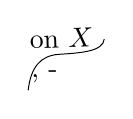
\begin{tikzpicture}[x=1em,y=1em,baseline=(b.base)]
\node[anchor=base west,inner sep=0] (b) at (0,0) {, -};
\node[anchor=base west,inner sep=0,rotate=2] at (-.05,1.05) {\inserted{\handwritten{on $X$}}};
\draw[line width=.35pt] (-.1,-.45) .. controls (.0,.4) and (.35,.8) .. (1.0,.85) .. controls (1.8,.9) and (2.6,.95) .. (2.65,1.4);
\end{tikzpicture}} in fact, one must restrict oneself here to \uline{chain} complexes), using the theory of \mbox{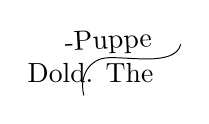
\begin{tikzpicture}[x=1em,y=1em,baseline=(b.base)]
\node[anchor=base west,inner sep=0] (b) at (0,0) {Dold. The};
\node[anchor=base west,inner sep=0,rotate=3] at (1.35,1.15) {\inserted{\handwritten{-Puppe}}};
\draw[line width=.35pt] (2.05,-.45) .. controls (1.85,.35) and (2.35,.85) .. (2.8,.9) .. controls (3.5,1.0) and (5.35,.55) .. (5.55,1.4);
\end{tikzpicture}} serious difficulty consisted in proving that these operations in $K^\bullet(X)$ satisfy the usual algebraic properties, allowing one to express for example $\handwritten{\lambda}^i(xy)$ as a universal polynomial with integer coefficients in the $\handwritten{\lambda}^j(x),\handwritten{\lambda}^k(y)$. Deligne proceeds by a very ingenious route, first determining the\unsure{\rlap{u}a|\rlap{a}u} $\handwritten{\lambda}$-ring structure of all the ``universal tensor op\rlap{\deleted{\unsure{a}}}erations'' that one can perform on vector bundles. \rlap{\deleted{\unsure{S|E}}}He has written his theory only when one works over a base field \deleted{\unsure{finite}}\handwritten{(}of arbitrary characteristic\handwritten{)}. \deleted{The case of characteristic}
% archive sheet number: 120
